\chapter{空间像素级细粒度感知：频空协同的大模型参数高效微调机制}

\section{引言}
在上一章中，本文针对机载边缘算力受限的客观物理条件，提出了 LiteFM-RSDet 实例级感知架构。该架构成功解决了广域巡航下的目标快速搜寻与宏观定位问题，使得无人机系统能够在海量的高分辨率遥感影像中，以极低的功耗实时“框定”感兴趣的潜在目标（如车辆、建筑物、桥梁等）。然而，宏观的实例级感知仅仅是空天视觉认知链路的第一步，面对真实且复杂的深水区解译任务，感知的粒度必须进一步下沉。

\subsection{灾害损毁评估中的微观拓扑提取需求}
在典型的城乡环境灾害损毁评估任务中（如地震致灾后的建筑形变分析、洪涝灾害中的基础设施阻断排查），受灾目标往往呈现出极度不规则的几何形变、碎片化的空间分布以及复杂的拓扑交错结构。在此背景下，单纯的实例级矩形框无法剥离目标内部的复杂环境背景，亦无法提供灾损量化评估所必需的高精度几何面积、形变比例与拓扑轮廓。

例如，在对半坍塌或受损建筑物进行精准定损时，系统必须剥离周围废墟的杂波干扰，精确提取残骸的像素级多边形边界。因此，视觉感知的研究范式必须从“实例级定位（Instance-level Localization）”跨越至“空间像素级分割（Pixel-level Segmentation）”。这就要求网络架构具备卓越的细粒度特征表达能力，以实现在高频纹理高度交织的城乡灾害背景中，划定高度贴合目标真实形态的物理边界。

\subsection{视觉大模型的迁移困境与灾害特征提取瓶颈}
为突破像素级精细化感知的瓶颈，近年来，以 Segment Anything Model (SAM) 为代表的视觉基础模型凭借其在海量数据上学习到的广义表征先验，在语义分割任务中展现出了卓越的性能（outstanding performance in semantic segmentation）。将此类通用视觉大模型引入遥感影像的灾害解译，已成为当前学术界的前沿趋势。

然而，遥感影像与自然场景图像在成像机理和物理特性上存在着显著的域间鸿沟。当尝试将这些先进的通用大模型直接应用于灾害区域提取任务时，模型面临着极其严峻的跨域适配挑战。具体而言，遥感灾害场景存在三大固有的视觉特征痛点：

极小的空间尺度（Small spatial scales）： 遥感视角下的损伤目标往往占据极少的像素区域，容易在深层网络的下采样过程中被平滑遗漏。

微弱的光谱差异（Weak spectral differences）： 受损地物（如破碎的水泥瓦砾）与其周围的自然背景（如裸土、沙石）在可见光波段的光谱反射率高度相似，极易造成语义混淆。

模糊的物理边界（Ambiguous boundaries）： 灾害导致的结构坍塌使得原本规则的人造物边缘变得支离破碎，难以提取连续且清晰的拓扑轮廓。

由于上述限制，通用大模型在识别跨越不同尺度的灾害专属特征（如结构性损伤、碎片分布模式等 disaster signatures: structural damage, debris patterns）时，往往会出现严重的边界溢出或特征丢失现象。

为了克服这些局限性，打通通用大模型向遥感灾害感知平滑迁移的理论链路，本文提出了一种全新的 SAM 适配框架——FourierPDC-SAM。该框架旨在通过极低成本的参数微调，构建互补的特征表征体系（complementary representations），在保留局部灾害特征响应的同时，稳健提取全局上下文信息，从而实现灾害区域的精细化像素级提取。

\begin{figure}[t]
  \centering
  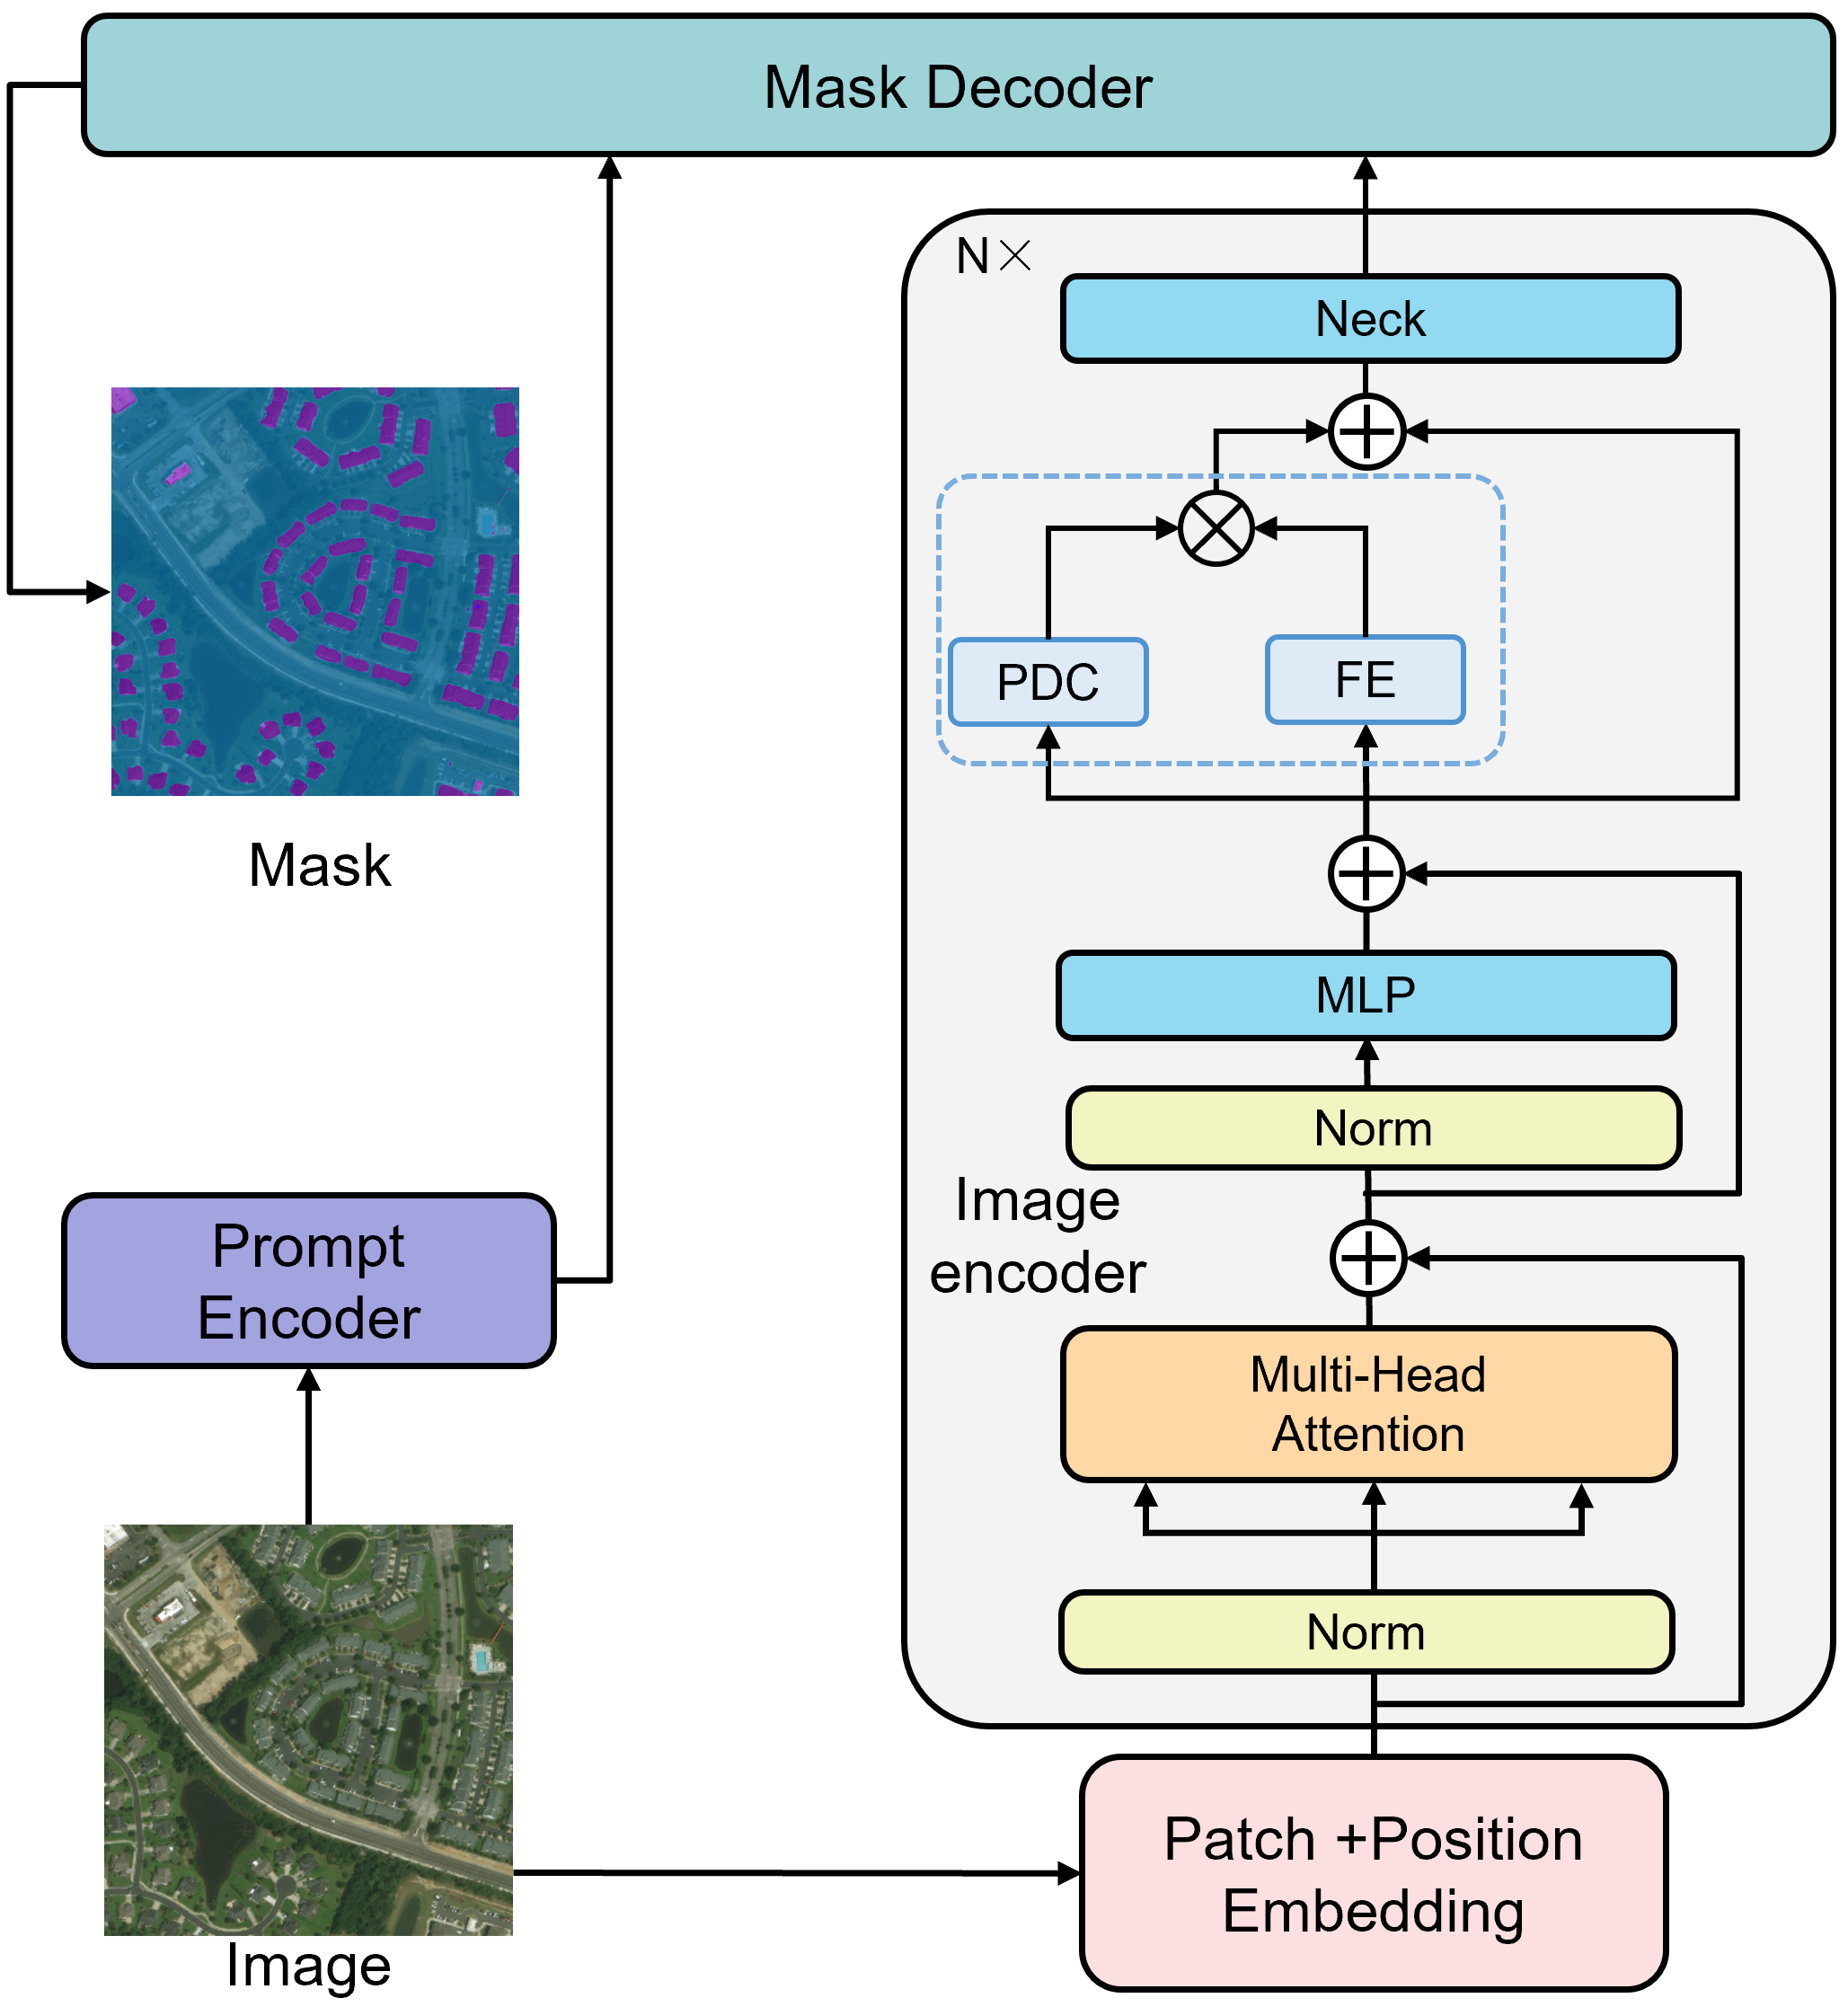
\includegraphics[width=.8\linewidth]{figures/FSAMstructure.png}
  \caption{FourierPDC-SAM架构图，展示了像素差分引导卷积和频域增强模块与标准SAM框架的融合，以提升灾后图像的分割性能。}
  \label{fig:FSAMstructure}
\end{figure}

\section{面向局部细节补偿的像素差分感知机制 (Pixel Difference Convolution, PDC)}
在视觉大模型（如 SAM）的编码器执行深层特征提取与激进下采样的过程中，包含目标微观拓扑结构的高频空间信息往往会被不可逆地平滑或滤除。为了在参数高效微调（PEFT）的框架下，从空间域（Spatial Domain）有效补偿这些流失的局部细节响应，本文在视觉大模型的编码器中创新性地引入了像素差分感知机制（Pixel Difference Convolution, PDC）。

\subsection{标准卷积在细粒度特征提取中的感受野局限性}
在典型的城乡灾害评估等复杂遥感应用中，受灾区域往往呈现出极具挑战性的视觉特征：微小的空间尺度（Small Spatial Scales）、微弱的光谱差异（Weak Spectral Differences）以及极度模糊的物理边界（Ambiguous Boundaries）。例如，建筑物表面的细微裂缝、散落的破碎瓦砾与周围完好的土壤或水泥地面在光谱反射率上高度相似。

\begin{figure}[t]
  \centering
  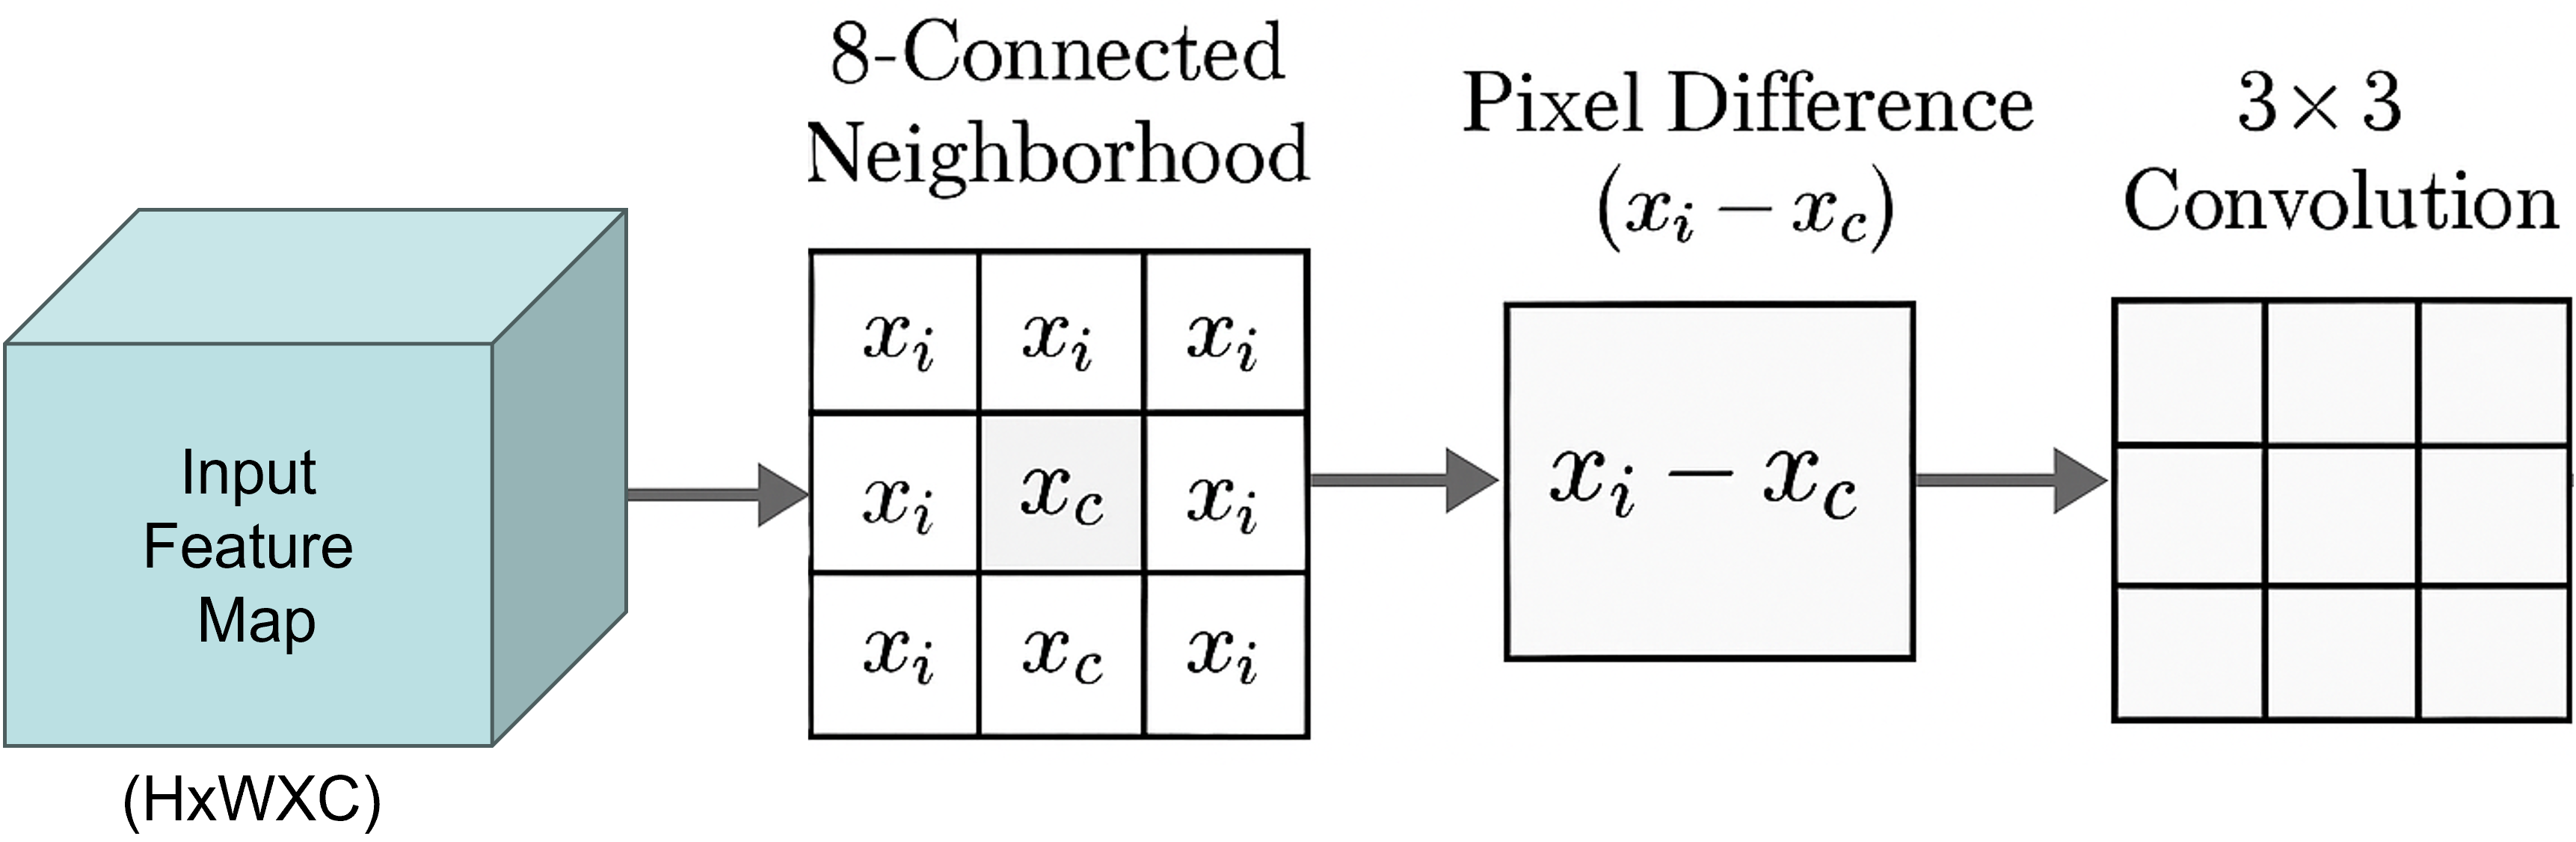
\includegraphics[width=.8\linewidth]{figures/PDC1.png}
  \caption{像素差分卷积（PDC）模块的结构。}
  \label{fig:PDC}
\end{figure}

传统的深度学习网络通常依赖标准卷积或常规的图块嵌入（Patch Embedding）算子来提取特征。然而，标准卷积的内积运算本质上是一种局部低通滤波器（Low-pass Filter），倾向于聚合邻域像素的共性而平滑局部差异。这种机制在面对灾害场景中细粒度的损伤模式（Fine-grained Damage Patterns）、低对比度边界（Low-contrast Boundaries）和高度破碎的结构（Fragmented Structures）时，往往会失效并导致严重的特征混淆。为了打破这一局限，系统迫切需要一种能够显式捕捉极微小空间突变的高频特征提取算子。

\subsection{像素级梯度聚合网络设计与微小拓扑特征捕获}
针对上述痛点，PDC 模块被设计为通过显式地对相邻位置的像素差值进行建模，从而精准捕获局部空间的变化梯度。这种像素级的差分计算机制对于检测遥感影像中极其隐蔽和细微的灾害损伤边界至关重要。PDC 的特征捕获过程首先从**差分计算（Difference Computation）**开始。在特征图的空间维度上，对于任意中心像素位置，算法提取其 8 连通邻域（8-Connected Neighborhood），即中心像素周围的 8 个方向偏移量，记为 $\{\Delta_k\}_{k=1}^8$。网络通过计算中心像素与其邻域像素在特征空间中的绝对差值，来提取各方向的局部梯度信息：$$D_k = X_{conv} - Shift(X_{conv}; \Delta_k), \quad k=1,2,...,8 \quad (1)$$其中，$X_{conv}$ 表示输入的局部空间特征；$Shift(\cdot; \Delta_k)$ 表示将特征图沿着 $\Delta_k$ 方向进行平移的操作；$D_k$ 即为在第 $k$ 个方向上捕获的局部边缘响应差异。为了综合评估该局部区域的拓扑突变程度，防止单一方向梯度的偶然性干扰，网络对这 8 个方向的差分响应进行了聚合处理。具体而言，分别利用求和（Summation）与最大值池化（Maximum Pooling）算子提取特征：$$D_{sum} = \sum_{k=1}^{8} D_k \quad (2)$$$$D_{max} = \max_{k=1}^{8} D_k \quad (3)$$通过上述聚合操作，$D_{sum}$ 累积了局部的整体突变能量，而 $D_{max}$ 则锁定了局部最显著的高频边缘特征。

\subsection{基于 PDC 的空域高频信息补偿数学建模}
在提取并聚合了局部差分梯度后，系统需要对这些高频信息进行自适应筛选与空域特征重构，以实现对受损区域的高效辨识。首先，PDC 模块引入了**自适应注意力生成（Adaptive Attention Generation）**机制。将聚合后的求和差分特征 $D_{sum}$ 与最大值差分特征 $D_{max}$ 在通道维度（Channel-wise）上进行密集拼接，随后利用一个 $1\times 1$ 的卷积层进行通道降维与信息交互，并通过 Sigmoid 激活函数 $\sigma$ 生成动态的注意力权重矩阵 $A$：$$A = \sigma(Conv_{1\times 1}([D_{sum} || D_{max}])) \quad (4)$$其中，$[\cdot || \cdot]$ 表示通道维度的拼接操作。该注意力门控机制（Gated Mechanism）能够自适应地评估不同通道中高频边缘信息的重要性，赋予潜在损伤边界更高的响应权重。最后，执行空域特征增强（Spatial Enhancement）。将生成的注意力掩码 $A$ 与基础求和差分特征 $D_{sum}$ 进行逐元素加权，随后输入至内核大小为 $K=3$ 的深度可分离卷积（Depthwise Separable Convolution, $DWConv$）中进行感受野内的特征非线性映射：$$F_{pdc} = DWConv_{3\times 3}(A \odot D_{sum}) \quad (5)$$其中，$\odot$ 表示逐元素相乘；最终输出的增强特征张量 $F_{pdc} \in \mathbb{R}^{B \times (C \times K^2) \times H \times W}$ 成功实现了维度的扩展与语义的升维。通过上述严密的数学建模，PDC 模块在不引入庞大计算负担的前提下，成功捕获并重建了遥感灾害检测所必需的详尽边界与纹理结构信息（Detailed Boundary and Texture Information）。这种空域高频信息的定向补偿，为后续与全局频域特征的跨域协同奠定了坚实的微观拓扑基础。

\section{抑制复杂背景干扰的频域全局增强策略 (Frequency Enhancement, FE)}
在前一节中，像素差分感知机制（PDC）成功实现了局部空间突变的微观特征提取。然而，面对灾害遥感影像，仅依赖空间域的局部感知仍具有局限性。灾害损伤通常表现出跨越不同空间频率的多尺度特征 。这些特征的跨度极大，既包含了表征细粒度结构裂缝的高频信号，也包含了表征大范围破坏模式的低频信号 。为了全面捕捉这些全局光谱模式，本文在空间域 PDC 模块之外，并行引入了频域全局增强（Frequency-domain Enhancement, FE）处理机制 。

\begin{figure}[t]
  \centering
  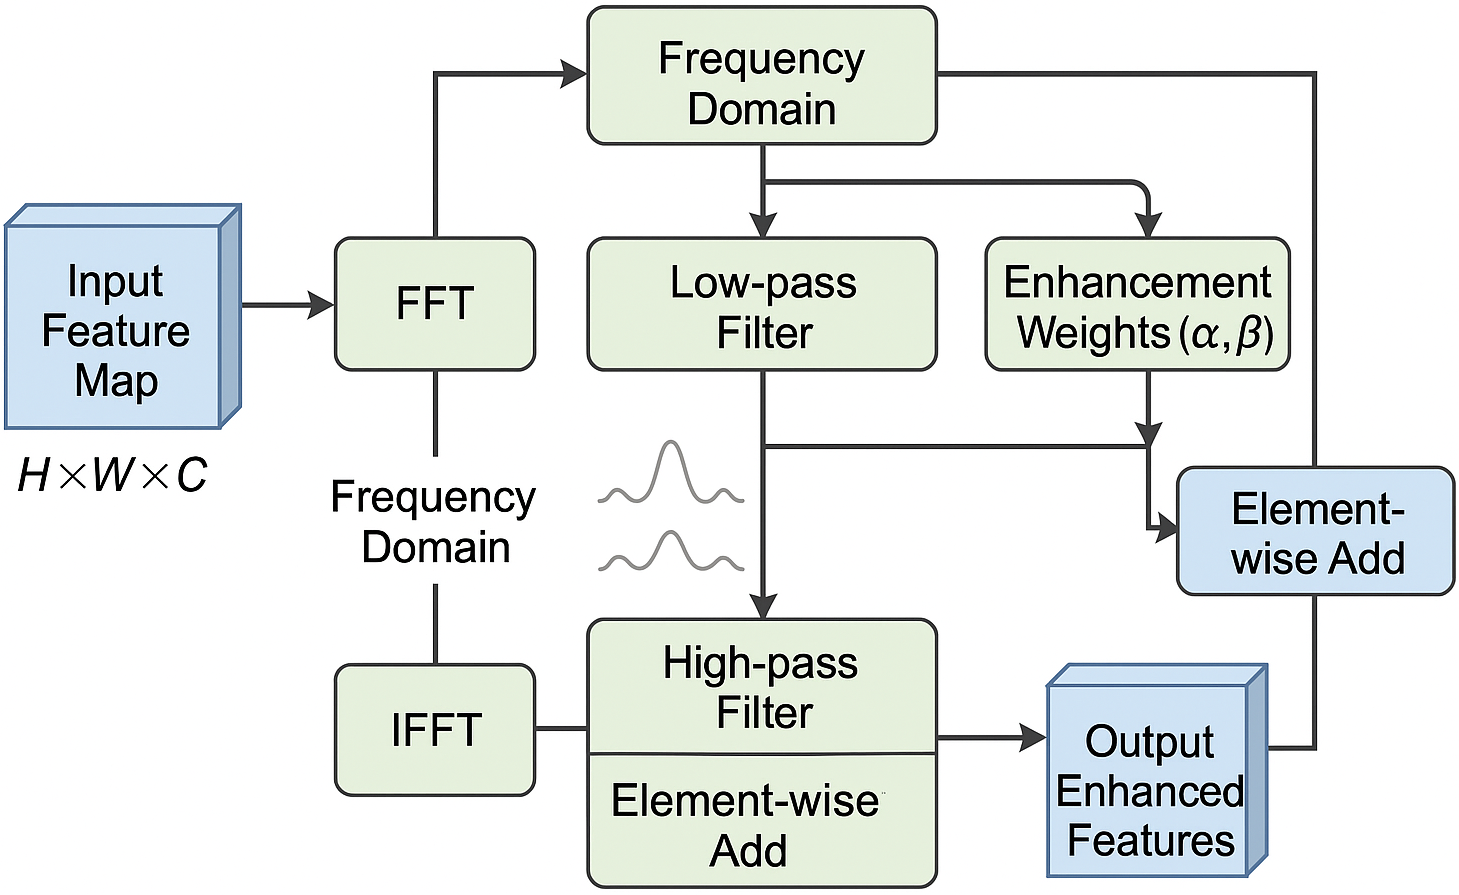
\includegraphics[width=.8\linewidth]{figures/FE.png}
  \caption{频域增强（FE）模块的结构。}
  \label{fig:FE}
\end{figure}

\subsection{空间域复杂形态的拓扑混淆与光谱相近性难题}
在城乡灾害损毁评估中，受损区域往往表现出极高的复杂性：微小的空间尺度、碎片化的分布以及与背景极低的光谱对比度。特别是受损的废墟残骸与自然裸土在可见光空间域的光谱特征高度相近，导致空间域卷积算子极易产生拓扑混淆。

空间域的卷积操作主要依赖局部感受野，难以在全局视野下区分噪声与结构主体。相反，在频域空间中，图像的全局空间分布模式会被转化为不同频率成分的能量分布：平坦的背景和宏观破坏主体通常集中在低频区域，而复杂的边缘、裂缝与散落的碎片则表现为高频分量。因此，通过频域变换将空间特征解耦为多尺度的频谱响应，是突破空间域光谱相近性瓶颈、实现全局特征增强的必由之路。

\subsection{傅里叶频域变换与多尺度频带解耦算子设计}
为了实现上述目标，FE 模块首先执行频率变换（Frequency Transformation）。系统将空间特征提取网络输出的特征图转换至频域，并计算其对数幅度谱 ：
$$\hat{X} = \mathcal{F}(X_{conv}) \quad (5)$$$$S = \log(1 + |\hat{X}|) \quad (6)$$其中，$\mathcal{F}$ 表示二维快速傅里叶变换（2D Fast Fourier Transform, FFT），$S \in \mathbb{R}^{B \times C \times H \times W}$ 代表计算得到的对数幅度谱 。引入对数变换（Logarithmic transformation）的数学意义在于，它不仅能够显著增强网络在反向传播中的数值稳定性，还能有效放大并强调那些极其微弱的频谱变化 。在获取了对数幅度谱后，系统进入**频带分析（Frequency Band Analysis）**阶段。本文根据特征点距离直流分量（DC Component，即代表图像平均强度的中心频率）的径向距离，将整个频率平面划分为 $B=4$ 个同心环状频带，集合记为 $\{\mathcal{B}_b\}_{b=1}^B$ 。
这 4 个频带在物理意义上严格对应着不同的空间尺度特性 。具体而言，从内部频带（Band 1）向外部频带（Band 4）过渡，其所代表的空间频率逐渐升高，分别捕获从宏观结构到微观裂缝的多层次纹理 。
在划分完毕的每一个频带内部，网络计算其平均频谱响应作为该频带的全局统计量 ：
$$g_b = \frac{1}{|\mathcal{B}_b|} \sum_{(u,v) \in \mathcal{B}_b} S(u,v), \quad b=1,2,...,B \quad (7)$$其中，$|\mathcal{B}_b|$ 表示第 $b$ 个频带内包含的频率分量总数 。通过这一公式，系统将高维的二维频谱映射为了一组低维且极具代表性的频带统计特征 。4.3.3 频域全局振幅调制的数学推演与空域重构获取了各个频带的平均响应 $g_b$ 后，为了使得网络能够自适应地关注（或抑制）特定频段的能量（例如放大高频损伤边缘、抑制低频背景噪声），FE 模块引入了**自适应频率加权（Adaptive Frequency Weighting）**机制 。系统采用了一个包含 2 个隐藏层的轻量级多层感知机（MLP）来处理提取到的频带统计信息，进而预测出逐通道的注意力权重 ：
$$w_b = \sigma(MLP(g_b)) \quad (8)$$$$\tilde{S}(u,v) = w_{b(u,v)} \cdot S(u,v) \quad (9)$$在上述推导中，$w_b \in \mathbb{R}^C$ 表示网络学习到的注意力权重向量；映射函数 $b(u,v)$ 的作用是将二维频率坐标 $(u,v)$ 精确映射回其所属的频带索引；$\tilde{S}(u,v)$ 则为经过全局振幅调制后的增强频谱 。最后，网络必须执行**空域恢复（Spatial Domain Recovery）**操作，将调制后的频域信号逆变换回空间域供后续大模型编码器使用 。在这一逆变换过程中，极其关键的一步是必须严格保留原始特征的相位信息（Phase Information），因为相位携带着目标的结构位置与几何拓扑先验 ：
$$\tilde{\hat{X}} = \tilde{S} \cdot e^{j \angle \hat{X}} \quad (10)$$$$F_{freq} = Real(\mathcal{F}^{-1}(\tilde{\hat{X}})) \quad (11)$$其中，$j$ 代表复数域的虚数单位，$\angle \hat{X}$ 用于从原始傅里叶频谱中提取真实的相位信息，$\mathcal{F}^{-1}$ 表示二维逆快速傅里叶变换（Inverse FFT）算子，$Real(\cdot)$ 表示取复数的实部 。通过这一套严密的频域增强与逆变换重构闭环，FE 模块在完全不破坏原始空间拓扑的前提下，成功实现了对受灾场景多尺度全局纹理模式的高保真提取与背景噪声的深度抑制。这一频域特征 $F_{freq}$ 将与前一节提取的空域特征 $F_{pdc}$ 形成完美的维度互补。

\section{频空双维协同的轻量化适配器架构重构 (FourierPDC-Adapter)}
在分别通过像素差分卷积（PDC）和频域全局增强（FE）模块获取了灾害场景的微观局部突变与宏观全局频谱特征后，接下来的核心挑战在于：如何以极低的计算成本，将这两种跨域特征无缝注入到预训练的视觉大模型中，实现细粒度语义的有效补偿。为此，本文设计了 FourierPDC-SAM 架构，通过构建频空协同的轻量化适配器（Adapter），完成了大模型向遥感灾害领域的参数高效适配。
\subsection{参数高效微调（PEFT）范式的引入与网络冻结策略}
在模型整体架构的设计上，FourierPDC-SAM 严格保持了原始 Segment Anything Model (SAM) 的标准三组件拓扑：图像编码器（Image Encoder）、提示编码器（Prompt Encoder）以及掩码解码器（Mask Decoder）。

为了在提升细粒度灾害特征提取能力的同时，兼顾边缘设备的计算资源限制，本文引入了参数高效微调（Parameter-Efficient Fine-Tuning, PEFT）范式。具体而言，本文的结构修改被严格排他性地限制在图像编码器（Image Encoder）内部。通过将空间-频率特征增强机制仅嵌入到视觉 Transformer（ViT）编码器的特定选择层中，网络不仅成功保留了对现有各类 SAM 下游应用与提示工程（Prompting）的完美兼容性，同时极大程度地维持了前向推理的计算效率。在训练阶段，大模型的原始主干权重被冻结，系统仅通过反向传播优化 PDC、FE 及其融合模块中极其有限的增量参数。

\subsection{频空双分支特征的乘法门控跨域融合}
PDC 模块擅长捕捉局部的空间几何突变，而 FE 模块则专注于捕获全局的频率纹理模式，这两者在物理意义上构成了灾害特征签名的正交互补维度（Complementary aspects of disaster signatures）。在将这两股异质特征信息进行融合时，传统的做法通常是采用简单的加法融合（Additive Fusion）或通道拼接（Concatenation）。然而，简单的加法融合无法在数学上有效建模空间与频率特征之间的乘法交互效应（Multiplicative Interactions）。而这种非线性的乘法交互，对于网络准确识别城乡环境中高度复杂的结构损伤模式至关重要。因此，本文摒弃了常规的线性叠加，创新性地提出了一种**乘法门控融合（Multiplicative Gating Fusion）**机制。系统利用乘法交互来聚合这两类互补特征：$$F_{fused} = X_{conv} \odot (1 + \alpha \cdot F_{pdc}) \odot (1 + \beta \cdot F_{freq}) \quad (12)$$其中，$X_{conv}$ 为主干网络输入的基础特征张量，$\odot$ 表示逐元素相乘（Hadamard Product），$F_{fused}$ 为跨域融合后的综合特征张量。公式中的 $\alpha$ 和 $\beta$ 分别代表空间特征与频率特征的可学习缩放参数（Learnable scaling parameters），在网络初始化阶段被保守地设定为 $\alpha=0.1$ 和 $\beta=0.1$。这一缩放因子用于动态控制不同域增强信号对主特征的贡献权重。更为精妙的是，上述 $(1 + \cdot)$ 的残差乘法公式设计，在数学上提供了一层安全保障：当网络在浅层尚未学习到有效的增强特征，或针对某些简单区域（增强贡献趋近于 0）时，乘子项将退化为 1，从而无损地保留原始主干特征 $X_{conv}$，这极大地维护了模型微调早期的梯度传播与训练稳定性（Maintaining training stability）。

\subsection{维度投影对齐与残差级联集成机制}
在完成了乘法门控融合后，特征张量 $F_{fused}$ 包含了极高密度的频空增强语义，但其特征分布域已与预训练的 ViT 主干产生偏移。为此，系统需要执行维度投影对齐（Dimension Projection），通过一系列变换管道将其映射回原始维度空间：$$F_{proj} = Conv_{1\times 1}(LayerNorm2d(GELU(F_{fused}))) \in \mathbb{R}^{B \times C \times H \times W} \quad (13)$$如上式所示，融合特征依次通过了 GELU 非线性激活函数以增强表达能力、二维层归一化（LayerNorm2d）以平滑内部协方差偏移，最后由 $1\times 1$ 点云卷积（$Conv_{1\times 1}$）实现通道维度的精确投影与对齐。最后，为了实现与通用大模型的无缝对接，系统执行残差级联集成（Residual Integration）。经过投影的特征张量首先进行格式转换（Format Conversion），将其形状通过 $Permute$ 操作严格对齐回 ViT 编码器所要求的张量格式，并通过带有缩放系数的残差连接注入回主干网络：$$X_{out} = X_{mlp} + \gamma \cdot Permute(F_{proj})^{[B,H,W,C]} \quad (14)$$其中，$X_{mlp}$ 为 ViT 编码器内部 MLP 层的输出特征，$\gamma$ 为残差集成系数。为防止增强特征对大模型原有先验知识造成过度扰动，参数 $\gamma$ 在初始化时被设定为 $0.5$，用于在训练初始阶段平滑地控制注入特征的初始贡献量。通过上述“提取-融合-对齐-注入”的完整适配器重构流程，FourierPDC-SAM 以极低的训练成本，成功让视觉大模型具备了在遥感灾害影像中提取精细化多边形掩码（Mask）的高频感知能力。

\section{实验验证与精细化像素分割效能评估}
为了全面验证所提出的 FourierPDC-SAM 架构在复杂灾害场景下提取微观拓扑轮廓的有效性，并量化频空双维协同机制对视觉大模型的性能增益，本节在真实的灾害遥感基准数据集上开展了详尽的定量评价、消融剖析与定性可视化分析。

\subsection{实验数据集与预处理配置}
本章的像素级分割实验主要依托于国际权威的灾害评估基准数据集 xBD benchmark 展开。该数据集专门针对灾后场景中受损建筑物的提取与损伤分级任务而构建，涵盖了全球多种典型自然灾害（如地震、海啸、飓风等），是评估模型灾害应急响应与细粒度提取能力的理想平台。实验任务与数据预处理：本实验聚焦于单时相灾害后区域提取任务（Single-temporal post-disaster region extraction）。在数据预处理阶段，为了在保持高分辨率空间特征与适应网络硬件输入限制之间取得最佳平衡，所有输入的遥感图像均被统一缩放或边缘填充（Resized/padded）至 $1024 \times 1024$ 的空间尺寸。在网络推理阶段生成最终掩码时，系统通过对解码器输出的对数几率（Decoder logits）应用固定阈值 $\tau=0.5$ 来获取最终的二值化预测掩码（Binary masks）。

\subsection{评价指标体系}
为了严格且多维度地评估大模型在微调状态下的像素级分割质量，本文采用语义分割领域公认的四大核心评价指标：交并比（Intersection-over-Union, IoU）、Dice系数（等效于 F1 分数）、精确率（Precision）以及召回率（Recall）。所有的性能指标均在图像的原始分辨率下进行计算，以确保评估结果能够真实反映模型在实际工程部署中的像素级精度。在定义公式前，首先基于预测掩码与真实标签（Ground Truth）的像素级比对结果，定义混淆矩阵的四个基本统计量：真正例（True Positive, $TP$）、假正例（False Positive, $FP$）、假反例（False Negative, $FN$）和真反例（True Negative, $TN$）。1. 精确率 (Precision)：精确率衡量了模型预测为“受灾区域”的像素中，真正属于受灾区域的比例。其数学定义为：$$Precision = \frac{TP}{TP + FP}$$在应急响应场景中，精确率的大幅提升意味着假阳性（False Positives，即误报）的显著降低。这一点具有决定性的实战价值，因为过多的误报会导致极其宝贵的救援资源被错误配置（Misallocation of rescue resources）。2. 召回率 (Recall)：召回率衡量了所有真实的“受灾区域”像素中，被模型成功正确预测出来的比例。其数学定义为：$$Recall = \frac{TP}{TP + FN}$$3. Dice 系数 / F1 分数 (Dice/F1-Score)：Dice 系数是精确率和召回率的调和平均数，用于综合评价模型在正负样本极其不均衡的灾害场景下的整体分割性能。其数学定义为：$$Dice = \frac{2 \times Precision \times Recall}{Precision + Recall} = \frac{2 \times TP}{2 \times TP + FP + FN}$$4. 交并比 (Intersection-over-Union, IoU)：IoU 是语义分割中最严苛的核心指标，衡量了预测掩码集合与真实标签集合之间的重叠度。IoU 的提升在物理意义上直接等效于系统能够更加精准地描摹灾害影响区域的物理边界。其数学定义为：$$IoU = \frac{TP}{TP + FP + FN}$$实验的比较基准（Baseline）设定为未经过频空域适配的原始视觉基础大模型 Segment Anything Model (SAM)。

\subsection{像素级分割精度定量分析与应急响应效能}
为了直观展示频空协同适配器对基础大模型的性能驱动，表 1 汇总了 FourierPDC-SAM 与原始 SAM 在 xBD 数据集上的全局定量测试结果。

\begin{table}[htbp]
\centering
\caption{FourierPDC-SAM与原始SAM在xBD数据集上的整体性能对比。}
\label{tab:performance_xbd}
\begin{tabular}{l c c c c}
\toprule
Model & IoU & Dice/F1 & Precision & Recall \\
\midrule
SAM                            & 0.7043 & 0.8221 & 0.8139 & 0.8387 \\
+PDC                           & 0.7120 & 0.8270 & 0.8230 & 0.8370 \\
+FE                            & 0.7200 & 0.8328 & 0.8370 & 0.8350 \\
\textbf{Ours (FourierPDC-SAM)} & \textbf{0.7276} & \textbf{0.8386} & \textbf{0.8511} & \textbf{0.8322} \\
\bottomrule
\end{tabular}
\end{table}

测试数据表明，原始 SAM 模型在灾害场景下的 IoU 仅为 0.7043，Dice 分数为 0.8221，精确率为 0.8139。引入本文提出的频空双维协同机制后，完整架构（FourierPDC-SAM）实现了全方位的性能跃升：

边界贴合度显著提升： 核心指标 IoU 从 0.7043 大幅提升至 0.7276（实现了 3.3\% 的相对提升）。Dice 分数也从 0.8221 同步提升至 0.8386（相对提升 2.0\%）。

高精确率与受控的折中： 模型的精确率实现了最大幅度的跨越，从 0.8139 跃升至 0.8511（相对提升 4.6\%）。与此同时，召回率仅出现微小的回落（从 0.8387 微降至 0.8322）。这种表现指示了一种极其“受控的权衡（Controlled trade-off）”。模型在大幅减少假阳性误报的同时，依然维持了极高水平的目标覆盖能力。这种精确率与 IoU 的协同优化，使得本方法在实际应用中能够有效避免不必要的误报，为灾害评估提供了极其可靠的工具。

\subsection{频空双维算子的正交消融实验与架构寻优}
为了量化剥离空间差分建模（PDC）、频域增强（FE）以及融合策略对大模型的独立贡献，本文设计了详尽的组件级消融实验（Ablation Study）。

\begin{table}[htbp]
\centering
\caption{关于FourierPDC-SAM组件的消融实验。}
\label{tab:ablation_fourierpdc_sam}
\begin{tabular}{c l c c c c}
\toprule
ID & Variant & IoU & Dice/F1 & Precision & Recall \\
\midrule
A & SAM (baseline)                   & 0.7043 & 0.8221 & 0.8139 & 0.8387 \\
B & +PDC only                        & 0.7120 & 0.8270 & 0.8230 & 0.8370 \\
C & +FE only                         & 0.7160 & 0.8280 & 0.8375 & 0.8247 \\
D & PDC + FE (additive fusion)       & 0.7192 & 0.8299 & 0.8433 & 0.8206 \\
\textbf{E} & \textbf{Ours: PDC + FE (multiplicative)} & \textbf{0.7276} & \textbf{0.8386} & \textbf{0.8511} & \textbf{0.8322} \\
F & w/o pixel difference in PDC      & 0.7075 & 0.8235 & 0.8185 & 0.8379 \\
G & Linear spectrum (no log scaling) & 0.7215 & 0.8321 & 0.8450 & 0.8221 \\
\bottomrule
\end{tabular}
\end{table}

频空单分支的有效性解耦： 以原始 SAM 为基准（变体 A，IoU 0.7043）。单独挂载像素差分引导卷积（+PDC only，变体 B）将 IoU 提升至 0.7120；而单独挂载傅里叶增强分支（+FE only，变体 C）将 IoU 提升至 0.7160。这表明 PDC 与 FE 均能有效提升基础 SAM 的性能，其中频域增强（FE）展现出略优的增益效果。然而，任何单一组件均无法企及完整频空双分支协同模型（变体 E，IoU 0.7276）的性能峰值。

跨域融合策略寻优： 在融合两大异质特征时，采用常规的加法融合（Additive fusion，变体 D）仅取得 0.7192 的 IoU。而本文提出的乘法门控融合策略（Multiplicative fusion，变体 E）则以 0.7276 的 IoU 取得了显著优势。这强有力地证明了：显式地对空间和频率特征之间的乘法交互效应（Multiplicative interactions）进行建模，对于识别复杂的灾害破坏模式至关重要。

底层算子设计的微观消融： 进一步深入模块内部细节，如果移除 PDC 模块中核心的显式像素差分计算（变体 F），系统 IoU 会骤降至 0.7075。同理，如果在 FE 模块中放弃对数幅度缩放，转而使用线性频谱（Linear spectrum，变体 G），IoU 会回落至 0.7215。这两项实验确认了本文核心架构设计在捕获微妙的灾害特征签名（Subtle disaster signatures）时的不可或缺性。

\subsection{细粒度轮廓重构的定性可视化分析}
为了直观解析 FourierPDC-SAM 在微观拓扑提取上的视觉机理，本文选取了两个具有代表性的城市灾害场景进行了定性可视化对比。

\begin{figure}[t]
  \centering
  \includegraphics[width=.8\linewidth]{figures/result.png}
  \caption{在两个具有代表性的城市场景上的定性比较。在相同的提示和阈值下，与原始SAM相比，FourierPDC-SAM在细节上表现更优（如屋顶边缘更清晰、相邻区域分离更准确、噪声更少等）。}
  \label{fig:SAMresult}
\end{figure}

在给定完全相同的提示（Identical prompts）与二值化阈值的严格控制下，FourierPDC-SAM 展现出了压倒性的细节描摹优势：

高频边缘的精准重构： 在目标损伤特征对比度低且空间分布稀疏的区域，FourierPDC-SAM 的边界锐利度（Boundary sharpness）得到了显著提升。它能够比原始 SAM 更好地勾勒出模糊暗淡的边缘（Faint edges）以及细小的碎片化损伤（Small fragmented damage）。此外，模型在提取建筑物屋顶边缘（Clearer roof edges）时也展现出了极高的几何贴合度。

复杂背景杂波的深度抑制： 得益于频空协同机制，FourierPDC-SAM 有效压制了周围环境的纹理杂波干扰（Suppressing background clutter），实现了更优的邻域地物分离（Better neighborhood separation），输出了极其干净、噪点极少（Fewer noises）的精细分割掩码。

这些直观的可视化证据与前文定量测试中更高精确率和交并比的结论高度吻合，从表象层面完美证实了该微调架构在解决通用大模型“高频边界模糊”痛点上的有效性。

\section{讨论与结论}
本章针对实例级宏观定位在复杂城乡灾害评估中无法提供精确多边形轮廓的局限性，以及通用视觉基础大模型（如 SAM）在遥感域迁移中面临的“高频边界流失”与“微调算力灾难”难题，提出了一种频空双维协同的大模型参数高效微调架构——FourierPDC-SAM。本章的核心工作与理论贡献可凝练为以下三个方面：

揭示并补偿了视觉大模型的空间降采样拓扑缺陷： 深入剖析了 SAM 等通用大模型在提取细粒度遥感灾害特征时产生“边界模糊”的底层机理。为此，创新性地提出了像素差分感知机制（PDC），通过显式计算局部邻域的像素级空间梯度，精准重构了因网络激进下采样而流失的微小受损地物高频边界与微观物理拓扑。

构建了频空正交的灾害特征解耦与重构范式： 针对灾区废墟与自然背景光谱高度混淆的难题，跳出单一空间域的局限，引入了基于傅里叶变换的全局频域增强策略（FE）。通过对多尺度频带的全局振幅调制，有效滤除了复杂环境下的相似背景杂波。进一步地，提出了乘法门控融合机制，将微观空间突变与宏观频率纹理进行非线性交叉融合，从数学机理上完善了复杂灾害破坏模式的表征体系。

实现了低算力下的精细化像素级解译效能跃升： 在 xBD 灾害评估基准数据集上的广泛实验表明，该架构在仅微调极少量增量参数（PEFT 范式）的条件下，实现了分割精度的全面超越。相比于原始 SAM，核心指标 IoU 显著提升了 3.3\%，精确率（Precision）大幅提升了 4.6\%。这一“受控的权衡”不仅有效抑制了灾害应急响应中的假阳性误报，更在定性可视化中展现了对不规则受损边界的极致描摹能力，为灾损定量分析提供了高可靠性的像素级解译工具。

下一章导读（局限性探讨与拓展）：

尽管基于可见光影像的空间像素级细粒度感知已在灾害拓扑提取上取得了突破性进展，但视觉大模型的表征上限依然受制于可见光光学成像的物理天花板。在真实的极端灾害场景中，目标往往面临极其复杂的环境干扰：例如受损地物被浓密烟雾遮蔽、被泥石流或洪区水体完全覆盖，亦或是处于夜间及极端恶劣天气条件。

当目标地物的表观可见光光学特征被彻底破坏或掩盖时，单纯依赖空间形态与可见光纹理的像素级提取模型将面临“特征失效”的认知极限。为了穿透这种维度的盲区，实现全天候、全天时的地物属性鉴别与深层次解译，感知系统必须打破单一可见光波段的桎梏，引入具备物理穿透性与材质反演能力的多模态数据（如 SAR 雷达影像）或高光谱数据。

因此，下一章将跳出可见光空间域的感知范畴，逻辑主线将向多模态/光谱级深度融合感知延伸，探讨如何在更为恶劣的物理遮挡环境下，利用多源异构数据协同，实现对复杂灾害目标的深层属性解译与稳健识别。